\documentclass[twoside]{book}

% Packages required by doxygen
\usepackage{fixltx2e}
\usepackage{calc}
\usepackage{doxygen}
\usepackage[export]{adjustbox} % also loads graphicx
\usepackage{graphicx}
\usepackage[utf8]{inputenc}
\usepackage{makeidx}
\usepackage{multicol}
\usepackage{multirow}
\PassOptionsToPackage{warn}{textcomp}
\usepackage{textcomp}
\usepackage[nointegrals]{wasysym}
\usepackage[table]{xcolor}

% Font selection
\usepackage[T1]{fontenc}
\usepackage[scaled=.90]{helvet}
\usepackage{courier}
\usepackage{amssymb}
\usepackage{sectsty}
\renewcommand{\familydefault}{\sfdefault}
\allsectionsfont{%
  \fontseries{bc}\selectfont%
  \color{darkgray}%
}
\renewcommand{\DoxyLabelFont}{%
  \fontseries{bc}\selectfont%
  \color{darkgray}%
}
\newcommand{\+}{\discretionary{\mbox{\scriptsize$\hookleftarrow$}}{}{}}

% Page & text layout
\usepackage{geometry}
\geometry{%
  a4paper,%
  top=2.5cm,%
  bottom=2.5cm,%
  left=2.5cm,%
  right=2.5cm%
}
\tolerance=750
\hfuzz=15pt
\hbadness=750
\setlength{\emergencystretch}{15pt}
\setlength{\parindent}{0cm}
\setlength{\parskip}{3ex plus 2ex minus 2ex}
\makeatletter
\renewcommand{\paragraph}{%
  \@startsection{paragraph}{4}{0ex}{-1.0ex}{1.0ex}{%
    \normalfont\normalsize\bfseries\SS@parafont%
  }%
}
\renewcommand{\subparagraph}{%
  \@startsection{subparagraph}{5}{0ex}{-1.0ex}{1.0ex}{%
    \normalfont\normalsize\bfseries\SS@subparafont%
  }%
}
\makeatother

% Headers & footers
\usepackage{fancyhdr}
\pagestyle{fancyplain}
\fancyhead[LE]{\fancyplain{}{\bfseries\thepage}}
\fancyhead[CE]{\fancyplain{}{}}
\fancyhead[RE]{\fancyplain{}{\bfseries\leftmark}}
\fancyhead[LO]{\fancyplain{}{\bfseries\rightmark}}
\fancyhead[CO]{\fancyplain{}{}}
\fancyhead[RO]{\fancyplain{}{\bfseries\thepage}}
\fancyfoot[LE]{\fancyplain{}{}}
\fancyfoot[CE]{\fancyplain{}{}}
\fancyfoot[RE]{\fancyplain{}{\bfseries\scriptsize 構築\+: Doxygen }}
\fancyfoot[LO]{\fancyplain{}{\bfseries\scriptsize 構築\+: Doxygen }}
\fancyfoot[CO]{\fancyplain{}{}}
\fancyfoot[RO]{\fancyplain{}{}}
\renewcommand{\footrulewidth}{0.4pt}
\renewcommand{\chaptermark}[1]{%
  \markboth{#1}{}%
}
\renewcommand{\sectionmark}[1]{%
  \markright{\thesection\ #1}%
}

% Indices & bibliography
\usepackage{natbib}
\usepackage[titles]{tocloft}
\setcounter{tocdepth}{3}
\setcounter{secnumdepth}{5}
\makeindex

% Hyperlinks (required, but should be loaded last)
\usepackage{ifpdf}
\ifpdf
  \usepackage[pdftex,pagebackref=true]{hyperref}
\else
  \usepackage[ps2pdf,pagebackref=true]{hyperref}
\fi
\hypersetup{%
  colorlinks=true,%
  linkcolor=blue,%
  citecolor=blue,%
  unicode%
}

% Custom commands
\newcommand{\clearemptydoublepage}{%
  \newpage{\pagestyle{empty}\cleardoublepage}%
}

\usepackage{caption}
\captionsetup{labelsep=space,justification=centering,font={bf},singlelinecheck=off,skip=4pt,position=top}

%===== C O N T E N T S =====

\begin{document}

% Titlepage & ToC
\hypersetup{pageanchor=false,
             bookmarksnumbered=true,
             pdfencoding=unicode
            }
\pagenumbering{alph}
\begin{titlepage}
\vspace*{7cm}
\begin{center}%
{\Large My Project }\\
\vspace*{1cm}
{\large 構築\+: Doxygen 1.8.14}\\
\end{center}
\end{titlepage}
\clearemptydoublepage
\pagenumbering{roman}
\tableofcontents
\clearemptydoublepage
\pagenumbering{arabic}
\hypersetup{pageanchor=true}

%--- Begin generated contents ---
\chapter{階層索引}
\section{クラス階層}
クラス階層一覧です。大雑把に文字符号順で並べられています。\begin{DoxyCompactList}
\item \contentsline{section}{C\+H\+A\+N\+N\+EL}{\pageref{class_c_h_a_n_n_e_l}}{}
\begin{DoxyCompactList}
\item \contentsline{section}{A\+BC}{\pageref{class_a_b_c}}{}
\item \contentsline{section}{D\+EF}{\pageref{class_d_e_f}}{}
\end{DoxyCompactList}
\item \contentsline{section}{List}{\pageref{class_list}}{}
\item \contentsline{section}{List\+Item}{\pageref{class_list_item}}{}
\begin{DoxyCompactList}
\item \contentsline{section}{Weather\+Record}{\pageref{class_weather_record}}{}
\end{DoxyCompactList}
\item \contentsline{section}{TV}{\pageref{class_t_v}}{}
\end{DoxyCompactList}

\chapter{クラス索引}
\section{クラス一覧}
クラス・構造体・共用体・インターフェースの一覧です。\begin{DoxyCompactList}
\item\contentsline{section}{\hyperlink{class_a_b_c}{A\+BC} }{\pageref{class_a_b_c}}{}
\item\contentsline{section}{\hyperlink{class_c_h_a_n_n_e_l}{C\+H\+A\+N\+N\+EL} }{\pageref{class_c_h_a_n_n_e_l}}{}
\item\contentsline{section}{\hyperlink{class_d_e_f}{D\+EF} }{\pageref{class_d_e_f}}{}
\item\contentsline{section}{\hyperlink{class_list}{List} }{\pageref{class_list}}{}
\item\contentsline{section}{\hyperlink{class_list_item}{List\+Item} }{\pageref{class_list_item}}{}
\item\contentsline{section}{\hyperlink{class_t_v}{TV} }{\pageref{class_t_v}}{}
\item\contentsline{section}{\hyperlink{class_weather_record}{Weather\+Record} }{\pageref{class_weather_record}}{}
\end{DoxyCompactList}

\chapter{ファイル索引}
\section{File List}
Here is a list of all files with brief descriptions\+:\begin{DoxyCompactList}
\item\contentsline{section}{\hyperlink{button__getdata_8c}{button\+\_\+getdata.\+c} }{\pageref{button__getdata_8c}}{}
\item\contentsline{section}{\hyperlink{button__getdata_8h}{button\+\_\+getdata.\+h} }{\pageref{button__getdata_8h}}{}
\item\contentsline{section}{\hyperlink{button__main_8c}{button\+\_\+main.\+c} }{\pageref{button__main_8c}}{}
\item\contentsline{section}{\hyperlink{button__out_8c}{button\+\_\+out.\+c} }{\pageref{button__out_8c}}{}
\item\contentsline{section}{\hyperlink{button__out_8h}{button\+\_\+out.\+h} }{\pageref{button__out_8h}}{}
\item\contentsline{section}{\hyperlink{common_8h}{common.\+h} }{\pageref{common_8h}}{}
\end{DoxyCompactList}

\chapter{クラス詳解}
\hypertarget{class_a_b_c}{}\section{A\+BC クラス}
\label{class_a_b_c}\index{A\+BC@{A\+BC}}


A\+BC の継承関係図\nopagebreak
\begin{figure}[H]
\begin{center}
\leavevmode
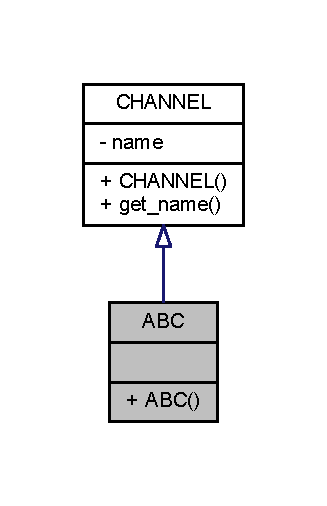
\includegraphics[width=157pt]{class_a_b_c__inherit__graph}
\end{center}
\end{figure}


A\+BC 連携図\nopagebreak
\begin{figure}[H]
\begin{center}
\leavevmode
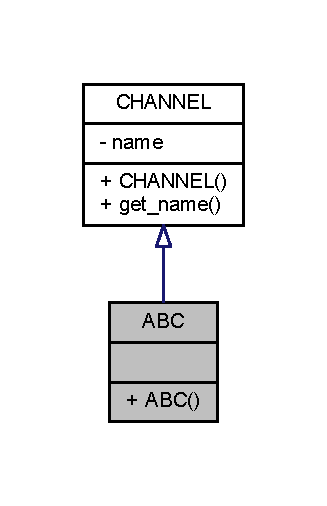
\includegraphics[width=157pt]{class_a_b_c__coll__graph}
\end{center}
\end{figure}
\subsection*{公開メンバ関数}
\begin{DoxyCompactItemize}
\item 
\hyperlink{class_a_b_c_a1bea7fc9f73e0d6878f9d2ac9ef3c1ec}{A\+BC} ()
\end{DoxyCompactItemize}


\subsection{詳解}


 chanel.\+cpp の 21 行目に定義があります。



\subsection{構築子と解体子}
\mbox{\Hypertarget{class_a_b_c_a1bea7fc9f73e0d6878f9d2ac9ef3c1ec}\label{class_a_b_c_a1bea7fc9f73e0d6878f9d2ac9ef3c1ec}} 
\index{A\+BC@{A\+BC}!A\+BC@{A\+BC}}
\index{A\+BC@{A\+BC}!A\+BC@{A\+BC}}
\subsubsection{\texorpdfstring{A\+B\+C()}{ABC()}}
{\footnotesize\ttfamily A\+B\+C\+::\+A\+BC (\begin{DoxyParamCaption}{ }\end{DoxyParamCaption})\hspace{0.3cm}{\ttfamily [inline]}}



 chanel.\+cpp の 23 行目に定義があります。


\begin{DoxyCode}
23 :\hyperlink{class_c_h_a_n_n_e_l_a233c9484f865fee53d66da81fb6b9e2d}{CHANNEL}(\textcolor{stringliteral}{"ABC局"})\{\}
\end{DoxyCode}


このクラス詳解は次のファイルから抽出されました\+:\begin{DoxyCompactItemize}
\item 
\hyperlink{chanel_8cpp}{chanel.\+cpp}\end{DoxyCompactItemize}

\hypertarget{class_c_h_a_n_n_e_l}{}\section{C\+H\+A\+N\+N\+EL クラス}
\label{class_c_h_a_n_n_e_l}\index{C\+H\+A\+N\+N\+EL@{C\+H\+A\+N\+N\+EL}}


C\+H\+A\+N\+N\+EL の継承関係図\nopagebreak
\begin{figure}[H]
\begin{center}
\leavevmode
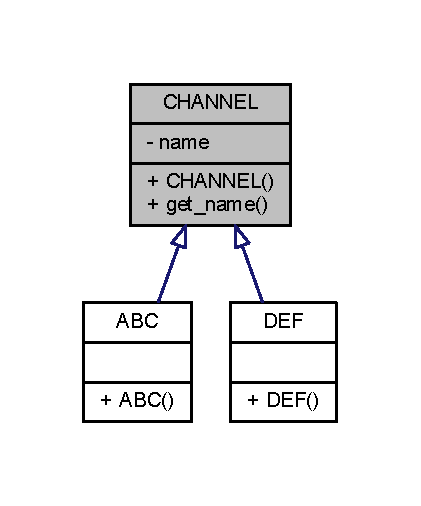
\includegraphics[width=202pt]{class_c_h_a_n_n_e_l__inherit__graph}
\end{center}
\end{figure}


C\+H\+A\+N\+N\+EL 連携図\nopagebreak
\begin{figure}[H]
\begin{center}
\leavevmode
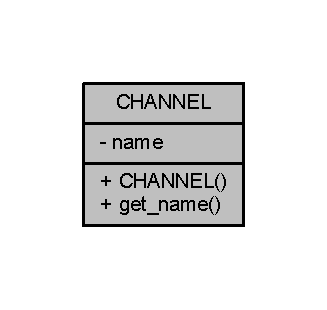
\includegraphics[width=157pt]{class_c_h_a_n_n_e_l__coll__graph}
\end{center}
\end{figure}
\subsection*{公開メンバ関数}
\begin{DoxyCompactItemize}
\item 
\hyperlink{class_c_h_a_n_n_e_l_a233c9484f865fee53d66da81fb6b9e2d}{C\+H\+A\+N\+N\+EL} (std\+::string input)
\item 
std\+::string \hyperlink{class_c_h_a_n_n_e_l_aa9daccb6ddb609e501245fed29f0adfd}{get\+\_\+name} ()
\end{DoxyCompactItemize}
\subsection*{非公開変数類}
\begin{DoxyCompactItemize}
\item 
std\+::string \hyperlink{class_c_h_a_n_n_e_l_a1a513303b0e58b1c9e0e9e03f9f50617}{name}
\end{DoxyCompactItemize}


\subsection{詳解}


 chanel.\+cpp の 8 行目に定義があります。



\subsection{構築子と解体子}
\mbox{\Hypertarget{class_c_h_a_n_n_e_l_a233c9484f865fee53d66da81fb6b9e2d}\label{class_c_h_a_n_n_e_l_a233c9484f865fee53d66da81fb6b9e2d}} 
\index{C\+H\+A\+N\+N\+EL@{C\+H\+A\+N\+N\+EL}!C\+H\+A\+N\+N\+EL@{C\+H\+A\+N\+N\+EL}}
\index{C\+H\+A\+N\+N\+EL@{C\+H\+A\+N\+N\+EL}!C\+H\+A\+N\+N\+EL@{C\+H\+A\+N\+N\+EL}}
\subsubsection{\texorpdfstring{C\+H\+A\+N\+N\+E\+L()}{CHANNEL()}}
{\footnotesize\ttfamily C\+H\+A\+N\+N\+E\+L\+::\+C\+H\+A\+N\+N\+EL (\begin{DoxyParamCaption}\item[{std\+::string}]{input }\end{DoxyParamCaption})\hspace{0.3cm}{\ttfamily [inline]}}



 chanel.\+cpp の 12 行目に定義があります。


\begin{DoxyCode}
12                             \{
13         this->\hyperlink{class_c_h_a_n_n_e_l_a1a513303b0e58b1c9e0e9e03f9f50617}{name} = input;
14     \}
\end{DoxyCode}


\subsection{関数詳解}
\mbox{\Hypertarget{class_c_h_a_n_n_e_l_aa9daccb6ddb609e501245fed29f0adfd}\label{class_c_h_a_n_n_e_l_aa9daccb6ddb609e501245fed29f0adfd}} 
\index{C\+H\+A\+N\+N\+EL@{C\+H\+A\+N\+N\+EL}!get\+\_\+name@{get\+\_\+name}}
\index{get\+\_\+name@{get\+\_\+name}!C\+H\+A\+N\+N\+EL@{C\+H\+A\+N\+N\+EL}}
\subsubsection{\texorpdfstring{get\+\_\+name()}{get\_name()}}
{\footnotesize\ttfamily std\+::string C\+H\+A\+N\+N\+E\+L\+::get\+\_\+name (\begin{DoxyParamCaption}{ }\end{DoxyParamCaption})\hspace{0.3cm}{\ttfamily [inline]}}



 chanel.\+cpp の 15 行目に定義があります。



参照先 name.



参照元 T\+V\+::change\+\_\+channel().


\begin{DoxyCode}
15                         \{
16         \textcolor{keywordflow}{return} this->\hyperlink{class_c_h_a_n_n_e_l_a1a513303b0e58b1c9e0e9e03f9f50617}{name};
17     \}
\end{DoxyCode}
被呼び出し関係図\+:\nopagebreak
\begin{figure}[H]
\begin{center}
\leavevmode
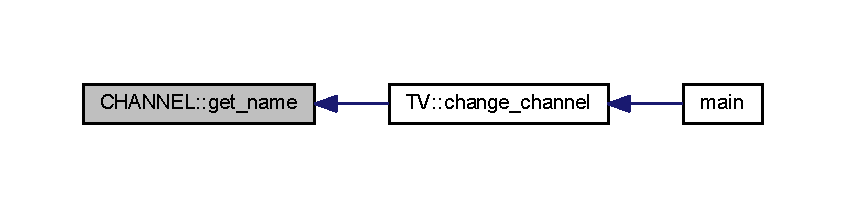
\includegraphics[width=350pt]{class_c_h_a_n_n_e_l_aa9daccb6ddb609e501245fed29f0adfd_icgraph}
\end{center}
\end{figure}


\subsection{メンバ詳解}
\mbox{\Hypertarget{class_c_h_a_n_n_e_l_a1a513303b0e58b1c9e0e9e03f9f50617}\label{class_c_h_a_n_n_e_l_a1a513303b0e58b1c9e0e9e03f9f50617}} 
\index{C\+H\+A\+N\+N\+EL@{C\+H\+A\+N\+N\+EL}!name@{name}}
\index{name@{name}!C\+H\+A\+N\+N\+EL@{C\+H\+A\+N\+N\+EL}}
\subsubsection{\texorpdfstring{name}{name}}
{\footnotesize\ttfamily std\+::string C\+H\+A\+N\+N\+E\+L\+::name\hspace{0.3cm}{\ttfamily [private]}}



 chanel.\+cpp の 10 行目に定義があります。



参照元 get\+\_\+name().



このクラス詳解は次のファイルから抽出されました\+:\begin{DoxyCompactItemize}
\item 
\hyperlink{chanel_8cpp}{chanel.\+cpp}\end{DoxyCompactItemize}

\hypertarget{class_d_e_f}{}\section{D\+EF クラス}
\label{class_d_e_f}\index{D\+EF@{D\+EF}}


D\+EF の継承関係図\nopagebreak
\begin{figure}[H]
\begin{center}
\leavevmode
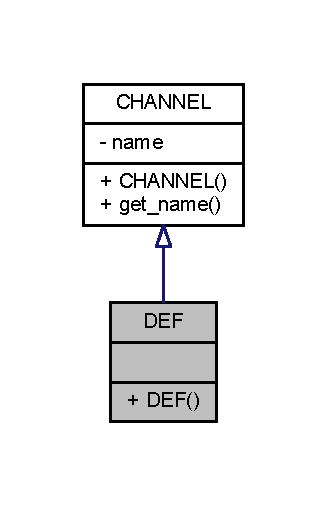
\includegraphics[width=157pt]{class_d_e_f__inherit__graph}
\end{center}
\end{figure}


D\+EF 連携図\nopagebreak
\begin{figure}[H]
\begin{center}
\leavevmode
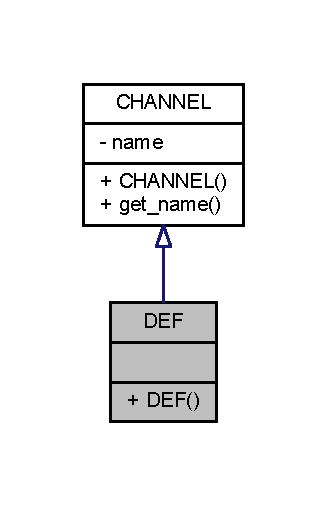
\includegraphics[width=157pt]{class_d_e_f__coll__graph}
\end{center}
\end{figure}
\subsection*{公開メンバ関数}
\begin{DoxyCompactItemize}
\item 
\hyperlink{class_d_e_f_a359a19dbba360787927e4a30485c6cde}{D\+EF} ()
\end{DoxyCompactItemize}


\subsection{詳解}


 chanel.\+cpp の 26 行目に定義があります。



\subsection{構築子と解体子}
\mbox{\Hypertarget{class_d_e_f_a359a19dbba360787927e4a30485c6cde}\label{class_d_e_f_a359a19dbba360787927e4a30485c6cde}} 
\index{D\+EF@{D\+EF}!D\+EF@{D\+EF}}
\index{D\+EF@{D\+EF}!D\+EF@{D\+EF}}
\subsubsection{\texorpdfstring{D\+E\+F()}{DEF()}}
{\footnotesize\ttfamily D\+E\+F\+::\+D\+EF (\begin{DoxyParamCaption}{ }\end{DoxyParamCaption})\hspace{0.3cm}{\ttfamily [inline]}}



 chanel.\+cpp の 28 行目に定義があります。


\begin{DoxyCode}
28 :\hyperlink{class_c_h_a_n_n_e_l_a233c9484f865fee53d66da81fb6b9e2d}{CHANNEL}(\textcolor{stringliteral}{"DEF局"})\{\}
\end{DoxyCode}


このクラス詳解は次のファイルから抽出されました\+:\begin{DoxyCompactItemize}
\item 
\hyperlink{chanel_8cpp}{chanel.\+cpp}\end{DoxyCompactItemize}

\hypertarget{class_list}{}\section{List クラス}
\label{class_list}\index{List@{List}}


List 連携図
% FIG 0
\subsection*{公開メンバ関数}
\begin{DoxyCompactItemize}
\item 
\hyperlink{class_list_a1fa6361e0cbcad09ed3e748b22eb1e19}{List} (int num)
\item 
\hyperlink{class_list_a70aecf37bd9d779a394e4d50377fbf5f}{$\sim$\+List} ()
\item 
void \hyperlink{class_list_a593e13086a1d135ac9efb530d26cd94b}{Add} (\hyperlink{class_list_item}{List\+Item} $\ast$p)
\item 
void \hyperlink{class_list_ac59284ff8d930a99616e9a13d49f92b4}{Sort} ()
\item 
void \hyperlink{class_list_a071cb188f9bb9bb8d1d79e6f939c586c}{Print} ()
\item 
void \hyperlink{class_list_a518ec1c2a0f0331d4f5fd5733e197d0c}{Search} (const char $\ast$input)
\end{DoxyCompactItemize}
\subsection*{非公開変数類}
\begin{DoxyCompactItemize}
\item 
\hyperlink{class_list_item}{List\+Item} $\ast$$\ast$ \hyperlink{class_list_a0fd821411e5922f1733b2afe207f6b28}{data}
\item 
int \hyperlink{class_list_ab03801c8c3765b381b45a306d34f5daa}{point}
\item 
int \hyperlink{class_list_a73fc93ef327ff5f4bb35fd628b658d50}{max}
\end{DoxyCompactItemize}


\subsection{詳解}


 test.\+cpp の 52 行目に定義があります。



\subsection{構築子と解体子}
\mbox{\Hypertarget{class_list_a1fa6361e0cbcad09ed3e748b22eb1e19}\label{class_list_a1fa6361e0cbcad09ed3e748b22eb1e19}} 
\index{List@{List}!List@{List}}
\index{List@{List}!List@{List}}
\subsubsection{\texorpdfstring{List()}{List()}}
{\footnotesize\ttfamily List\+::\+List (\begin{DoxyParamCaption}\item[{int}]{num }\end{DoxyParamCaption})\hspace{0.3cm}{\ttfamily [inline]}}



 test.\+cpp の 59 行目に定義があります。


\begin{DoxyCode}
59                  \{
60         \textcolor{comment}{/* データ数分メモリ確保 */}
61         this->\hyperlink{class_list_a0fd821411e5922f1733b2afe207f6b28}{data} = \textcolor{keyword}{new} \hyperlink{class_list_item}{ListItem} * [num];
62         \textcolor{comment}{/* 現在のポインタ位置 */}
63         this->\hyperlink{class_list_ab03801c8c3765b381b45a306d34f5daa}{point} = 0;
64         \textcolor{comment}{/* 最大サイズ */}
65         this->\hyperlink{class_list_a73fc93ef327ff5f4bb35fd628b658d50}{max} = num;
66     \}
\end{DoxyCode}
\mbox{\Hypertarget{class_list_a70aecf37bd9d779a394e4d50377fbf5f}\label{class_list_a70aecf37bd9d779a394e4d50377fbf5f}} 
\index{List@{List}!````~List@{$\sim$\+List}}
\index{````~List@{$\sim$\+List}!List@{List}}
\subsubsection{\texorpdfstring{$\sim$\+List()}{~List()}}
{\footnotesize\ttfamily List\+::$\sim$\+List (\begin{DoxyParamCaption}{ }\end{DoxyParamCaption})\hspace{0.3cm}{\ttfamily [inline]}}



 test.\+cpp の 68 行目に定義があります。


\begin{DoxyCode}
68            \{
69         \textcolor{keyword}{delete}[] this->\hyperlink{class_list_a0fd821411e5922f1733b2afe207f6b28}{data};
70     \}
\end{DoxyCode}


\subsection{関数詳解}
\mbox{\Hypertarget{class_list_a593e13086a1d135ac9efb530d26cd94b}\label{class_list_a593e13086a1d135ac9efb530d26cd94b}} 
\index{List@{List}!Add@{Add}}
\index{Add@{Add}!List@{List}}
\subsubsection{\texorpdfstring{Add()}{Add()}}
{\footnotesize\ttfamily void List\+::\+Add (\begin{DoxyParamCaption}\item[{\hyperlink{class_list_item}{List\+Item} $\ast$}]{p }\end{DoxyParamCaption})\hspace{0.3cm}{\ttfamily [inline]}}



 test.\+cpp の 72 行目に定義があります。



参照元 main().


\begin{DoxyCode}
72                          \{
73         \textcolor{comment}{/* データオーバー */}
74         \textcolor{keywordflow}{if}(this->\hyperlink{class_list_ab03801c8c3765b381b45a306d34f5daa}{point} >= this->\hyperlink{class_list_a73fc93ef327ff5f4bb35fd628b658d50}{max})\{
75             cout << \textcolor{stringliteral}{"memory size over"} << endl;
76             \textcolor{keywordflow}{return};
77         \}
78         \textcolor{comment}{/* データ格納 */}
79         \hyperlink{class_list_a0fd821411e5922f1733b2afe207f6b28}{data}[this->\hyperlink{class_list_ab03801c8c3765b381b45a306d34f5daa}{point}++] = p;
80         \textcolor{keywordflow}{return};
81     \}
\end{DoxyCode}
被呼び出し関係図\+:
% FIG 1
\mbox{\Hypertarget{class_list_a071cb188f9bb9bb8d1d79e6f939c586c}\label{class_list_a071cb188f9bb9bb8d1d79e6f939c586c}} 
\index{List@{List}!Print@{Print}}
\index{Print@{Print}!List@{List}}
\subsubsection{\texorpdfstring{Print()}{Print()}}
{\footnotesize\ttfamily void List\+::\+Print (\begin{DoxyParamCaption}{ }\end{DoxyParamCaption})\hspace{0.3cm}{\ttfamily [inline]}}



 test.\+cpp の 96 行目に定義があります。



参照先 List\+Item\+::\+Print().



参照元 main().


\begin{DoxyCode}
96                 \{
97         \textcolor{comment}{/* データ印字 */}
98         \textcolor{keywordflow}{for}(\textcolor{keywordtype}{int} loop = 0 ; loop < this->\hyperlink{class_list_ab03801c8c3765b381b45a306d34f5daa}{point}; loop++)\{
99             \hyperlink{class_list_a0fd821411e5922f1733b2afe207f6b28}{data}[loop]->\hyperlink{class_list_item_a0bb35843489312a6796d6f94f4395399}{Print}();
100         \}
101         \textcolor{keywordflow}{return};
102     \}
\end{DoxyCode}
呼び出し関係図\+:
% FIG 2
被呼び出し関係図\+:
% FIG 3
\mbox{\Hypertarget{class_list_a518ec1c2a0f0331d4f5fd5733e197d0c}\label{class_list_a518ec1c2a0f0331d4f5fd5733e197d0c}} 
\index{List@{List}!Search@{Search}}
\index{Search@{Search}!List@{List}}
\subsubsection{\texorpdfstring{Search()}{Search()}}
{\footnotesize\ttfamily void List\+::\+Search (\begin{DoxyParamCaption}\item[{const char $\ast$}]{input }\end{DoxyParamCaption})\hspace{0.3cm}{\ttfamily [inline]}}



 test.\+cpp の 104 行目に定義があります。



参照元 main().


\begin{DoxyCode}
104                                   \{
105         \textcolor{comment}{/* データ存在を確認 */}
106         \textcolor{keywordflow}{for}(\textcolor{keywordtype}{int} loop = 0 ; loop < this->\hyperlink{class_list_ab03801c8c3765b381b45a306d34f5daa}{point}; loop++)\{
107             \textcolor{comment}{/* データ存在 */}
108             \textcolor{keywordflow}{if}(!strcmp(input,\hyperlink{class_list_a0fd821411e5922f1733b2afe207f6b28}{data}[loop]->name))\{
109                 cout << input << \textcolor{stringliteral}{" is exist"} << endl;
110                 \textcolor{keywordflow}{return};
111             \}
112         \}
113         \textcolor{comment}{/* データ存在しない */}
114         cout << input << \textcolor{stringliteral}{" is not exist"} << endl;
115         \textcolor{keywordflow}{return};
116     \}
\end{DoxyCode}
被呼び出し関係図\+:
% FIG 4
\mbox{\Hypertarget{class_list_ac59284ff8d930a99616e9a13d49f92b4}\label{class_list_ac59284ff8d930a99616e9a13d49f92b4}} 
\index{List@{List}!Sort@{Sort}}
\index{Sort@{Sort}!List@{List}}
\subsubsection{\texorpdfstring{Sort()}{Sort()}}
{\footnotesize\ttfamily void List\+::\+Sort (\begin{DoxyParamCaption}{ }\end{DoxyParamCaption})\hspace{0.3cm}{\ttfamily [inline]}}



 test.\+cpp の 83 行目に定義があります。



参照先 swap().



参照元 main().


\begin{DoxyCode}
83                \{
84         \textcolor{comment}{/* ソートする */}
85         \textcolor{keywordflow}{for}(\textcolor{keywordtype}{int} loop = 0; loop < this->\hyperlink{class_list_ab03801c8c3765b381b45a306d34f5daa}{point} - 1; loop++)\{
86             \textcolor{keywordflow}{for}(\textcolor{keywordtype}{int} loop2 = this->point - 1 ; loop2 > loop ; loop2--)\{
87                 \textcolor{keywordflow}{if}(strcmp(this->\hyperlink{class_list_a0fd821411e5922f1733b2afe207f6b28}{data}[loop2]->name,this->\hyperlink{class_list_a0fd821411e5922f1733b2afe207f6b28}{data}[loop2 - 1]->name) < 0)\{
88                     \textcolor{comment}{/* スワップする */}
89                     \hyperlink{test_8cpp_add33a83c7b2de277d5846db56efc6dae}{swap}(this->\hyperlink{class_list_a0fd821411e5922f1733b2afe207f6b28}{data}[loop2],this->\hyperlink{class_list_a0fd821411e5922f1733b2afe207f6b28}{data}[loop2 -1]);
90                 \}
91             \}
92         \}
93         \textcolor{keywordflow}{return};
94     \}
\end{DoxyCode}
呼び出し関係図\+:
% FIG 5
被呼び出し関係図\+:
% FIG 6


\subsection{メンバ詳解}
\mbox{\Hypertarget{class_list_a0fd821411e5922f1733b2afe207f6b28}\label{class_list_a0fd821411e5922f1733b2afe207f6b28}} 
\index{List@{List}!data@{data}}
\index{data@{data}!List@{List}}
\subsubsection{\texorpdfstring{data}{data}}
{\footnotesize\ttfamily \hyperlink{class_list_item}{List\+Item}$\ast$$\ast$ List\+::data\hspace{0.3cm}{\ttfamily [private]}}



 test.\+cpp の 54 行目に定義があります。

\mbox{\Hypertarget{class_list_a73fc93ef327ff5f4bb35fd628b658d50}\label{class_list_a73fc93ef327ff5f4bb35fd628b658d50}} 
\index{List@{List}!max@{max}}
\index{max@{max}!List@{List}}
\subsubsection{\texorpdfstring{max}{max}}
{\footnotesize\ttfamily int List\+::max\hspace{0.3cm}{\ttfamily [private]}}



 test.\+cpp の 56 行目に定義があります。

\mbox{\Hypertarget{class_list_ab03801c8c3765b381b45a306d34f5daa}\label{class_list_ab03801c8c3765b381b45a306d34f5daa}} 
\index{List@{List}!point@{point}}
\index{point@{point}!List@{List}}
\subsubsection{\texorpdfstring{point}{point}}
{\footnotesize\ttfamily int List\+::point\hspace{0.3cm}{\ttfamily [private]}}



 test.\+cpp の 55 行目に定義があります。



このクラス詳解は次のファイルから抽出されました\+:\begin{DoxyCompactItemize}
\item 
\hyperlink{test_8cpp}{test.\+cpp}\end{DoxyCompactItemize}

\hypertarget{class_list_item}{}\section{List\+Item クラス}
\label{class_list_item}\index{List\+Item@{List\+Item}}


List\+Item の継承関係図
% FIG 0


List\+Item 連携図
% FIG 1
\subsection*{公開メンバ関数}
\begin{DoxyCompactItemize}
\item 
virtual void \hyperlink{class_list_item_a0bb35843489312a6796d6f94f4395399}{Print} ()=0
\item 
\hyperlink{class_list_item_a19fe16421201217d9c0647865243c07b}{List\+Item} (const char $\ast$\+\_\+date)
\end{DoxyCompactItemize}
\subsection*{公開変数類}
\begin{DoxyCompactItemize}
\item 
char $\ast$ \hyperlink{class_list_item_a721391bcdefb1a5f77b79295a80b0305}{name}
\end{DoxyCompactItemize}


\subsection{詳解}


 test.\+cpp の 7 行目に定義があります。



\subsection{構築子と解体子}
\mbox{\Hypertarget{class_list_item_a19fe16421201217d9c0647865243c07b}\label{class_list_item_a19fe16421201217d9c0647865243c07b}} 
\index{List\+Item@{List\+Item}!List\+Item@{List\+Item}}
\index{List\+Item@{List\+Item}!List\+Item@{List\+Item}}
\subsubsection{\texorpdfstring{List\+Item()}{ListItem()}}
{\footnotesize\ttfamily List\+Item\+::\+List\+Item (\begin{DoxyParamCaption}\item[{const char $\ast$}]{\+\_\+date }\end{DoxyParamCaption})\hspace{0.3cm}{\ttfamily [inline]}}



 test.\+cpp の 14 行目に定義があります。


\begin{DoxyCode}
14                                \{
15         \textcolor{comment}{/* 名前を初期化 */}
16         this->\hyperlink{class_list_item_a721391bcdefb1a5f77b79295a80b0305}{name} = \textcolor{keyword}{new} \textcolor{keywordtype}{char}[strlen(\_date) + 1];
17         memset( this->\hyperlink{class_list_item_a721391bcdefb1a5f77b79295a80b0305}{name} , \textcolor{charliteral}{'\(\backslash\)0'} , strlen( \_date ) + 1);
18         strcpy( this->\hyperlink{class_list_item_a721391bcdefb1a5f77b79295a80b0305}{name} , \_date );
19     \}
\end{DoxyCode}


\subsection{関数詳解}
\mbox{\Hypertarget{class_list_item_a0bb35843489312a6796d6f94f4395399}\label{class_list_item_a0bb35843489312a6796d6f94f4395399}} 
\index{List\+Item@{List\+Item}!Print@{Print}}
\index{Print@{Print}!List\+Item@{List\+Item}}
\subsubsection{\texorpdfstring{Print()}{Print()}}
{\footnotesize\ttfamily virtual void List\+Item\+::\+Print (\begin{DoxyParamCaption}{ }\end{DoxyParamCaption})\hspace{0.3cm}{\ttfamily [pure virtual]}}



\hyperlink{class_weather_record_a824790f08728d4deb81dfcbaec5a76ba}{Weather\+Record}で実装されています。



参照元 List\+::\+Print().

被呼び出し関係図\+:
% FIG 2


\subsection{メンバ詳解}
\mbox{\Hypertarget{class_list_item_a721391bcdefb1a5f77b79295a80b0305}\label{class_list_item_a721391bcdefb1a5f77b79295a80b0305}} 
\index{List\+Item@{List\+Item}!name@{name}}
\index{name@{name}!List\+Item@{List\+Item}}
\subsubsection{\texorpdfstring{name}{name}}
{\footnotesize\ttfamily char$\ast$ List\+Item\+::name}



 test.\+cpp の 9 行目に定義があります。



このクラス詳解は次のファイルから抽出されました\+:\begin{DoxyCompactItemize}
\item 
\hyperlink{test_8cpp}{test.\+cpp}\end{DoxyCompactItemize}

\hypertarget{class_t_v}{}\section{TV クラス}
\label{class_t_v}\index{TV@{TV}}


TV 連携図\nopagebreak
\begin{figure}[H]
\begin{center}
\leavevmode
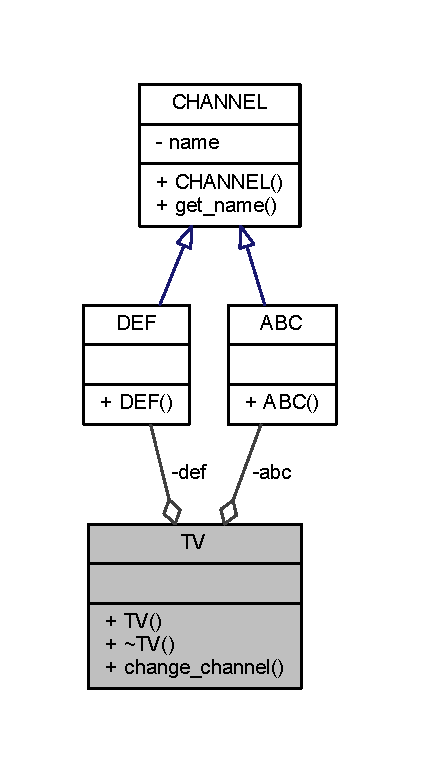
\includegraphics[width=202pt]{class_t_v__coll__graph}
\end{center}
\end{figure}
\subsection*{公開メンバ関数}
\begin{DoxyCompactItemize}
\item 
\hyperlink{class_t_v_a02a3fb40f0a254fef0b4aacb6362b563}{TV} ()
\item 
\hyperlink{class_t_v_a377383017c486aa83467f7ad977e3653}{$\sim$\+TV} ()
\item 
void \hyperlink{class_t_v_a26370b5928a57c9af9ed35f9c8f34ba4}{change\+\_\+channel} ()
\end{DoxyCompactItemize}
\subsection*{非公開変数類}
\begin{DoxyCompactItemize}
\item 
\hyperlink{class_a_b_c}{A\+BC} \hyperlink{class_t_v_a7bb8008571c1ca7539e937252503889b}{abc}
\item 
\hyperlink{class_d_e_f}{D\+EF} \hyperlink{class_t_v_ab5e13d7d33ed800b78ddb755b11b7fa2}{def}
\end{DoxyCompactItemize}


\subsection{詳解}


 chanel.\+cpp の 32 行目に定義があります。



\subsection{構築子と解体子}
\mbox{\Hypertarget{class_t_v_a02a3fb40f0a254fef0b4aacb6362b563}\label{class_t_v_a02a3fb40f0a254fef0b4aacb6362b563}} 
\index{TV@{TV}!TV@{TV}}
\index{TV@{TV}!TV@{TV}}
\subsubsection{\texorpdfstring{T\+V()}{TV()}}
{\footnotesize\ttfamily T\+V\+::\+TV (\begin{DoxyParamCaption}{ }\end{DoxyParamCaption})\hspace{0.3cm}{\ttfamily [inline]}}



 chanel.\+cpp の 37 行目に定義があります。


\begin{DoxyCode}
37         \{
38         std::cout << \textcolor{stringliteral}{"スイッチON\(\backslash\)n"};
39     \}
\end{DoxyCode}
\mbox{\Hypertarget{class_t_v_a377383017c486aa83467f7ad977e3653}\label{class_t_v_a377383017c486aa83467f7ad977e3653}} 
\index{TV@{TV}!````~TV@{$\sim$\+TV}}
\index{````~TV@{$\sim$\+TV}!TV@{TV}}
\subsubsection{\texorpdfstring{$\sim$\+T\+V()}{~TV()}}
{\footnotesize\ttfamily T\+V\+::$\sim$\+TV (\begin{DoxyParamCaption}{ }\end{DoxyParamCaption})\hspace{0.3cm}{\ttfamily [inline]}}



 chanel.\+cpp の 41 行目に定義があります。


\begin{DoxyCode}
41          \{
42         std::cout << \textcolor{stringliteral}{"スイッチOFF\(\backslash\)n"};
43     \}
\end{DoxyCode}


\subsection{関数詳解}
\mbox{\Hypertarget{class_t_v_a26370b5928a57c9af9ed35f9c8f34ba4}\label{class_t_v_a26370b5928a57c9af9ed35f9c8f34ba4}} 
\index{TV@{TV}!change\+\_\+channel@{change\+\_\+channel}}
\index{change\+\_\+channel@{change\+\_\+channel}!TV@{TV}}
\subsubsection{\texorpdfstring{change\+\_\+channel()}{change\_channel()}}
{\footnotesize\ttfamily void T\+V\+::change\+\_\+channel (\begin{DoxyParamCaption}{ }\end{DoxyParamCaption})\hspace{0.3cm}{\ttfamily [inline]}}



 chanel.\+cpp の 44 行目に定義があります。



参照先 A\+B\+C\+C\+H\+AN, D\+E\+F\+C\+H\+AN, C\+H\+A\+N\+N\+E\+L\+::get\+\_\+name(), O\+F\+F\+C\+H\+AN.



参照元 main().


\begin{DoxyCode}
44                          \{
45         std::cout << \textcolor{stringliteral}{"チャンネル入力 [ 0 or 1 or off ] : "};
46         std::string input;
47         std::cin >> input;
48         \textcolor{keywordflow}{if}(input == \hyperlink{chanel_8cpp_a513cb4309778b669aec8a3e5638079ac}{ABCCHAN})\{
49             std::cout << \hyperlink{class_t_v_a7bb8008571c1ca7539e937252503889b}{abc}.\hyperlink{class_c_h_a_n_n_e_l_aa9daccb6ddb609e501245fed29f0adfd}{get\_name}() << std::endl;
50         \}\textcolor{keywordflow}{else} \textcolor{keywordflow}{if}(input == \hyperlink{chanel_8cpp_aa9f5e75679b639a2c4ec2faf66372b86}{DEFCHAN})\{
51             std::cout << \hyperlink{class_t_v_ab5e13d7d33ed800b78ddb755b11b7fa2}{def}.\hyperlink{class_c_h_a_n_n_e_l_aa9daccb6ddb609e501245fed29f0adfd}{get\_name}() << std::endl;
52         \}\textcolor{keywordflow}{else} \textcolor{keywordflow}{if}(input == \hyperlink{chanel_8cpp_a0c1a83009ab44960907c64b7a1ad6135}{OFFCHAN})\{
53             \textcolor{keywordflow}{break};
54         \}
55     \}
\end{DoxyCode}
呼び出し関係図\+:\nopagebreak
\begin{figure}[H]
\begin{center}
\leavevmode
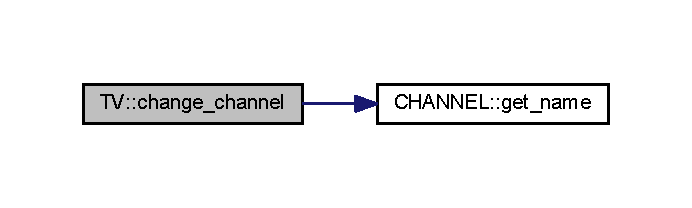
\includegraphics[width=332pt]{class_t_v_a26370b5928a57c9af9ed35f9c8f34ba4_cgraph}
\end{center}
\end{figure}
被呼び出し関係図\+:\nopagebreak
\begin{figure}[H]
\begin{center}
\leavevmode
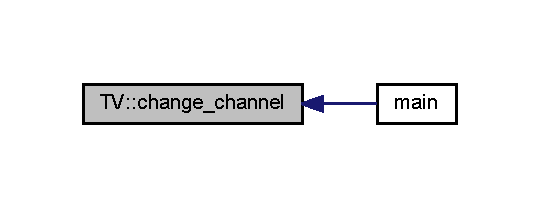
\includegraphics[width=259pt]{class_t_v_a26370b5928a57c9af9ed35f9c8f34ba4_icgraph}
\end{center}
\end{figure}


\subsection{メンバ詳解}
\mbox{\Hypertarget{class_t_v_a7bb8008571c1ca7539e937252503889b}\label{class_t_v_a7bb8008571c1ca7539e937252503889b}} 
\index{TV@{TV}!abc@{abc}}
\index{abc@{abc}!TV@{TV}}
\subsubsection{\texorpdfstring{abc}{abc}}
{\footnotesize\ttfamily \hyperlink{class_a_b_c}{A\+BC} T\+V\+::abc\hspace{0.3cm}{\ttfamily [private]}}



 chanel.\+cpp の 34 行目に定義があります。

\mbox{\Hypertarget{class_t_v_ab5e13d7d33ed800b78ddb755b11b7fa2}\label{class_t_v_ab5e13d7d33ed800b78ddb755b11b7fa2}} 
\index{TV@{TV}!def@{def}}
\index{def@{def}!TV@{TV}}
\subsubsection{\texorpdfstring{def}{def}}
{\footnotesize\ttfamily \hyperlink{class_d_e_f}{D\+EF} T\+V\+::def\hspace{0.3cm}{\ttfamily [private]}}



 chanel.\+cpp の 35 行目に定義があります。



このクラス詳解は次のファイルから抽出されました\+:\begin{DoxyCompactItemize}
\item 
\hyperlink{chanel_8cpp}{chanel.\+cpp}\end{DoxyCompactItemize}

\hypertarget{class_weather_record}{}\section{Weather\+Record クラス}
\label{class_weather_record}\index{Weather\+Record@{Weather\+Record}}


Weather\+Record の継承関係図
% FIG 0


Weather\+Record 連携図
% FIG 1
\subsection*{公開メンバ関数}
\begin{DoxyCompactItemize}
\item 
\hyperlink{class_weather_record_a6a4edf430381ee7ac701876f787c7633}{Weather\+Record} (const char $\ast$\+\_\+date, const char $\ast$\+\_\+weather, int \+\_\+high, int \+\_\+low)
\item 
void \hyperlink{class_weather_record_a824790f08728d4deb81dfcbaec5a76ba}{Print} ()
\end{DoxyCompactItemize}
\subsection*{非公開変数類}
\begin{DoxyCompactItemize}
\item 
char $\ast$ \hyperlink{class_weather_record_a3b9b2139f84c02e1ba36b1bee333e057}{weather}
\item 
int \hyperlink{class_weather_record_ab1f968211ccc7fe600f76d31f3b0edc9}{high}
\item 
int \hyperlink{class_weather_record_a16a7592e80388a4b2091c027cd18aed3}{low}
\end{DoxyCompactItemize}
\subsection*{その他の継承メンバ}


\subsection{詳解}


 test.\+cpp の 22 行目に定義があります。



\subsection{構築子と解体子}
\mbox{\Hypertarget{class_weather_record_a6a4edf430381ee7ac701876f787c7633}\label{class_weather_record_a6a4edf430381ee7ac701876f787c7633}} 
\index{Weather\+Record@{Weather\+Record}!Weather\+Record@{Weather\+Record}}
\index{Weather\+Record@{Weather\+Record}!Weather\+Record@{Weather\+Record}}
\subsubsection{\texorpdfstring{Weather\+Record()}{WeatherRecord()}}
{\footnotesize\ttfamily Weather\+Record\+::\+Weather\+Record (\begin{DoxyParamCaption}\item[{const char $\ast$}]{\+\_\+date,  }\item[{const char $\ast$}]{\+\_\+weather,  }\item[{int}]{\+\_\+high,  }\item[{int}]{\+\_\+low }\end{DoxyParamCaption})\hspace{0.3cm}{\ttfamily [inline]}}



 test.\+cpp の 29 行目に定義があります。


\begin{DoxyCode}
33              :\hyperlink{class_list_item_a19fe16421201217d9c0647865243c07b}{ListItem}(\_date)\{
34         \textcolor{comment}{/* 天気を初期化 */}
35         this->\hyperlink{class_weather_record_a3b9b2139f84c02e1ba36b1bee333e057}{weather} = \textcolor{keyword}{new} \textcolor{keywordtype}{char}[strlen(\_weather) + 1];
36         memset( this->\hyperlink{class_weather_record_a3b9b2139f84c02e1ba36b1bee333e057}{weather} , \textcolor{charliteral}{'\(\backslash\)0'} , strlen(\_weather) + 1);
37         strcpy( this->\hyperlink{class_weather_record_a3b9b2139f84c02e1ba36b1bee333e057}{weather} , \_weather);
38         \textcolor{comment}{/* 最高気温代入 */}
39         this->\hyperlink{class_weather_record_ab1f968211ccc7fe600f76d31f3b0edc9}{high} = \_high;
40         \textcolor{comment}{/* 最低気温代入 */}
41         this->\hyperlink{class_weather_record_a16a7592e80388a4b2091c027cd18aed3}{low} = \_low;
42     \}
\end{DoxyCode}


\subsection{関数詳解}
\mbox{\Hypertarget{class_weather_record_a824790f08728d4deb81dfcbaec5a76ba}\label{class_weather_record_a824790f08728d4deb81dfcbaec5a76ba}} 
\index{Weather\+Record@{Weather\+Record}!Print@{Print}}
\index{Print@{Print}!Weather\+Record@{Weather\+Record}}
\subsubsection{\texorpdfstring{Print()}{Print()}}
{\footnotesize\ttfamily void Weather\+Record\+::\+Print (\begin{DoxyParamCaption}{ }\end{DoxyParamCaption})\hspace{0.3cm}{\ttfamily [inline]}, {\ttfamily [virtual]}}



\hyperlink{class_list_item_a0bb35843489312a6796d6f94f4395399}{List\+Item}を実装しています。



 test.\+cpp の 44 行目に定義があります。


\begin{DoxyCode}
44                 \{
45         cout << this->\hyperlink{class_list_item_a721391bcdefb1a5f77b79295a80b0305}{name} << \textcolor{stringliteral}{": "} 
46         << this->\hyperlink{class_weather_record_a3b9b2139f84c02e1ba36b1bee333e057}{weather} << \textcolor{stringliteral}{": "} 
47         << this->\hyperlink{class_weather_record_ab1f968211ccc7fe600f76d31f3b0edc9}{high} << \textcolor{stringliteral}{"/"} << this->\hyperlink{class_weather_record_a16a7592e80388a4b2091c027cd18aed3}{low} << 
48         \textcolor{stringliteral}{"(度)"} << endl;
49     \}
\end{DoxyCode}


\subsection{メンバ詳解}
\mbox{\Hypertarget{class_weather_record_ab1f968211ccc7fe600f76d31f3b0edc9}\label{class_weather_record_ab1f968211ccc7fe600f76d31f3b0edc9}} 
\index{Weather\+Record@{Weather\+Record}!high@{high}}
\index{high@{high}!Weather\+Record@{Weather\+Record}}
\subsubsection{\texorpdfstring{high}{high}}
{\footnotesize\ttfamily int Weather\+Record\+::high\hspace{0.3cm}{\ttfamily [private]}}



 test.\+cpp の 25 行目に定義があります。

\mbox{\Hypertarget{class_weather_record_a16a7592e80388a4b2091c027cd18aed3}\label{class_weather_record_a16a7592e80388a4b2091c027cd18aed3}} 
\index{Weather\+Record@{Weather\+Record}!low@{low}}
\index{low@{low}!Weather\+Record@{Weather\+Record}}
\subsubsection{\texorpdfstring{low}{low}}
{\footnotesize\ttfamily int Weather\+Record\+::low\hspace{0.3cm}{\ttfamily [private]}}



 test.\+cpp の 26 行目に定義があります。

\mbox{\Hypertarget{class_weather_record_a3b9b2139f84c02e1ba36b1bee333e057}\label{class_weather_record_a3b9b2139f84c02e1ba36b1bee333e057}} 
\index{Weather\+Record@{Weather\+Record}!weather@{weather}}
\index{weather@{weather}!Weather\+Record@{Weather\+Record}}
\subsubsection{\texorpdfstring{weather}{weather}}
{\footnotesize\ttfamily char$\ast$ Weather\+Record\+::weather\hspace{0.3cm}{\ttfamily [private]}}



 test.\+cpp の 24 行目に定義があります。



このクラス詳解は次のファイルから抽出されました\+:\begin{DoxyCompactItemize}
\item 
\hyperlink{test_8cpp}{test.\+cpp}\end{DoxyCompactItemize}

\chapter{ファイル詳解}
\hypertarget{chanel_8cpp}{}\section{chanel.\+cpp ファイル}
\label{chanel_8cpp}\index{chanel.\+cpp@{chanel.\+cpp}}
{\ttfamily \#include $<$iostream$>$}\newline
{\ttfamily \#include $<$string$>$}\newline
chanel.\+cpp の依存先関係図\+:\nopagebreak
\begin{figure}[H]
\begin{center}
\leavevmode
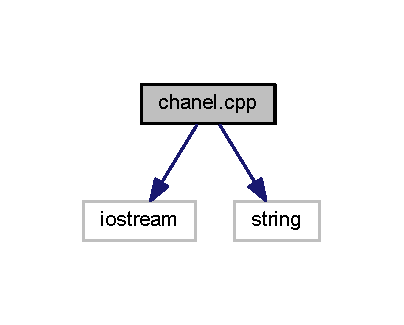
\includegraphics[width=194pt]{chanel_8cpp__incl}
\end{center}
\end{figure}
\subsection*{クラス}
\begin{DoxyCompactItemize}
\item 
class \hyperlink{class_c_h_a_n_n_e_l}{C\+H\+A\+N\+N\+EL}
\item 
class \hyperlink{class_a_b_c}{A\+BC}
\item 
class \hyperlink{class_d_e_f}{D\+EF}
\item 
class \hyperlink{class_t_v}{TV}
\end{DoxyCompactItemize}
\subsection*{マクロ定義}
\begin{DoxyCompactItemize}
\item 
\#define \hyperlink{chanel_8cpp_a513cb4309778b669aec8a3e5638079ac}{A\+B\+C\+C\+H\+AN}~\char`\"{}0\char`\"{}
\item 
\#define \hyperlink{chanel_8cpp_aa9f5e75679b639a2c4ec2faf66372b86}{D\+E\+F\+C\+H\+AN}~\char`\"{}1\char`\"{}
\item 
\#define \hyperlink{chanel_8cpp_a0c1a83009ab44960907c64b7a1ad6135}{O\+F\+F\+C\+H\+AN}~\char`\"{}O\+FF\char`\"{}
\end{DoxyCompactItemize}
\subsection*{関数}
\begin{DoxyCompactItemize}
\item 
int \hyperlink{chanel_8cpp_ae66f6b31b5ad750f1fe042a706a4e3d4}{main} ()
\end{DoxyCompactItemize}


\subsection{マクロ定義詳解}
\mbox{\Hypertarget{chanel_8cpp_a513cb4309778b669aec8a3e5638079ac}\label{chanel_8cpp_a513cb4309778b669aec8a3e5638079ac}} 
\index{chanel.\+cpp@{chanel.\+cpp}!A\+B\+C\+C\+H\+AN@{A\+B\+C\+C\+H\+AN}}
\index{A\+B\+C\+C\+H\+AN@{A\+B\+C\+C\+H\+AN}!chanel.\+cpp@{chanel.\+cpp}}
\subsubsection{\texorpdfstring{A\+B\+C\+C\+H\+AN}{ABCCHAN}}
{\footnotesize\ttfamily \#define A\+B\+C\+C\+H\+AN~\char`\"{}0\char`\"{}}



 chanel.\+cpp の 4 行目に定義があります。



参照元 T\+V\+::change\+\_\+channel().

\mbox{\Hypertarget{chanel_8cpp_aa9f5e75679b639a2c4ec2faf66372b86}\label{chanel_8cpp_aa9f5e75679b639a2c4ec2faf66372b86}} 
\index{chanel.\+cpp@{chanel.\+cpp}!D\+E\+F\+C\+H\+AN@{D\+E\+F\+C\+H\+AN}}
\index{D\+E\+F\+C\+H\+AN@{D\+E\+F\+C\+H\+AN}!chanel.\+cpp@{chanel.\+cpp}}
\subsubsection{\texorpdfstring{D\+E\+F\+C\+H\+AN}{DEFCHAN}}
{\footnotesize\ttfamily \#define D\+E\+F\+C\+H\+AN~\char`\"{}1\char`\"{}}



 chanel.\+cpp の 5 行目に定義があります。



参照元 T\+V\+::change\+\_\+channel().

\mbox{\Hypertarget{chanel_8cpp_a0c1a83009ab44960907c64b7a1ad6135}\label{chanel_8cpp_a0c1a83009ab44960907c64b7a1ad6135}} 
\index{chanel.\+cpp@{chanel.\+cpp}!O\+F\+F\+C\+H\+AN@{O\+F\+F\+C\+H\+AN}}
\index{O\+F\+F\+C\+H\+AN@{O\+F\+F\+C\+H\+AN}!chanel.\+cpp@{chanel.\+cpp}}
\subsubsection{\texorpdfstring{O\+F\+F\+C\+H\+AN}{OFFCHAN}}
{\footnotesize\ttfamily \#define O\+F\+F\+C\+H\+AN~\char`\"{}O\+FF\char`\"{}}



 chanel.\+cpp の 6 行目に定義があります。



参照元 T\+V\+::change\+\_\+channel().



\subsection{関数詳解}
\mbox{\Hypertarget{chanel_8cpp_ae66f6b31b5ad750f1fe042a706a4e3d4}\label{chanel_8cpp_ae66f6b31b5ad750f1fe042a706a4e3d4}} 
\index{chanel.\+cpp@{chanel.\+cpp}!main@{main}}
\index{main@{main}!chanel.\+cpp@{chanel.\+cpp}}
\subsubsection{\texorpdfstring{main()}{main()}}
{\footnotesize\ttfamily int main (\begin{DoxyParamCaption}{ }\end{DoxyParamCaption})}



 chanel.\+cpp の 58 行目に定義があります。



参照先 T\+V\+::change\+\_\+channel().


\begin{DoxyCode}
58           \{
59     \hyperlink{class_t_v}{TV} tv;
60     tv.\hyperlink{class_t_v_a26370b5928a57c9af9ed35f9c8f34ba4}{change\_channel}();
61     \textcolor{keywordflow}{return} 0;
62 \}
\end{DoxyCode}
呼び出し関係図\+:\nopagebreak
\begin{figure}[H]
\begin{center}
\leavevmode
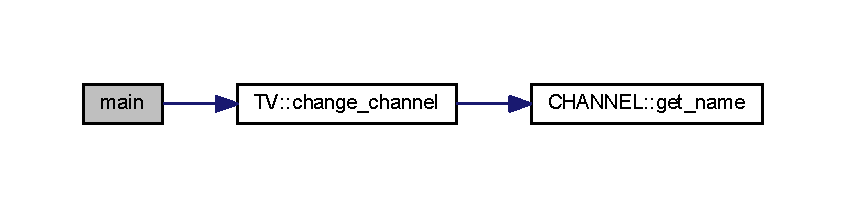
\includegraphics[width=350pt]{chanel_8cpp_ae66f6b31b5ad750f1fe042a706a4e3d4_cgraph}
\end{center}
\end{figure}

\hypertarget{test_8cpp}{}\section{test.\+cpp ファイル}
\label{test_8cpp}\index{test.\+cpp@{test.\+cpp}}
{\ttfamily \#include $<$iostream$>$}\newline
{\ttfamily \#include $<$string.\+h$>$}\newline
test.\+cpp の依存先関係図\+:
% FIG 0
\subsection*{クラス}
\begin{DoxyCompactItemize}
\item 
class \hyperlink{class_list_item}{List\+Item}
\item 
class \hyperlink{class_weather_record}{Weather\+Record}
\item 
class \hyperlink{class_list}{List}
\end{DoxyCompactItemize}
\subsection*{関数}
\begin{DoxyCompactItemize}
\item 
void \hyperlink{test_8cpp_add33a83c7b2de277d5846db56efc6dae}{swap} (char $\ast$input, char $\ast$input2)
\item 
int \hyperlink{test_8cpp_ae66f6b31b5ad750f1fe042a706a4e3d4}{main} ()
\end{DoxyCompactItemize}


\subsection{関数詳解}
\mbox{\Hypertarget{test_8cpp_ae66f6b31b5ad750f1fe042a706a4e3d4}\label{test_8cpp_ae66f6b31b5ad750f1fe042a706a4e3d4}} 
\index{test.\+cpp@{test.\+cpp}!main@{main}}
\index{main@{main}!test.\+cpp@{test.\+cpp}}
\subsubsection{\texorpdfstring{main()}{main()}}
{\footnotesize\ttfamily int main (\begin{DoxyParamCaption}{ }\end{DoxyParamCaption})}



 test.\+cpp の 126 行目に定義があります。



参照先 List\+::\+Add(), List\+::\+Print(), List\+::\+Search(), List\+::\+Sort().


\begin{DoxyCode}
126           \{
127 
128     \textcolor{keywordtype}{int} num;
129     \textcolor{comment}{/* データサイズ入力 */}
130     cout <<\textcolor{stringliteral}{"INPUT DATA SIZE:"} << endl;
131     cin >> num;
132     \textcolor{comment}{/* Listクラスのインスタンスの生成 */}
133     \hyperlink{class_list}{List} weatherlist(num);
134     \textcolor{comment}{/* エントリーの追加 */}
135     weatherlist.Add(\textcolor{keyword}{new} \hyperlink{class_weather_record}{WeatherRecord}(\textcolor{stringliteral}{"2015-06-24"}, \textcolor{stringliteral}{"sunny"}, 29, 18));
136     weatherlist.Add(\textcolor{keyword}{new} \hyperlink{class_weather_record}{WeatherRecord}(\textcolor{stringliteral}{"2015-06-25"}, \textcolor{stringliteral}{"cloudy"}, 29, 20));
137     weatherlist.Add(\textcolor{keyword}{new} \hyperlink{class_weather_record}{WeatherRecord}(\textcolor{stringliteral}{"2015-06-23"}, \textcolor{stringliteral}{"sunny"}, 27, 19));
138     weatherlist.Add(\textcolor{keyword}{new} \hyperlink{class_weather_record}{WeatherRecord}(\textcolor{stringliteral}{"2015-06-26"}, \textcolor{stringliteral}{"rain"}, 26, 19));
139     \textcolor{comment}{/* 印刷 */}
140     weatherlist.Print();
141     cout << \textcolor{stringliteral}{"-----------------"} << endl;
142     \textcolor{comment}{/* エントリーのソート */}
143     weatherlist.Sort();
144     \textcolor{comment}{/* 印刷 */}
145     weatherlist.Print();
146     cout << \textcolor{stringliteral}{"-----------------"} << endl;
147     \textcolor{comment}{/* 検索 */}
148     weatherlist.Search(\textcolor{stringliteral}{"2015-06-22"});
149     weatherlist.Search(\textcolor{stringliteral}{"2015-06-24"});
150     \textcolor{keywordflow}{return} 0;
151 \}
\end{DoxyCode}
呼び出し関係図\+:
% FIG 1
\mbox{\Hypertarget{test_8cpp_add33a83c7b2de277d5846db56efc6dae}\label{test_8cpp_add33a83c7b2de277d5846db56efc6dae}} 
\index{test.\+cpp@{test.\+cpp}!swap@{swap}}
\index{swap@{swap}!test.\+cpp@{test.\+cpp}}
\subsubsection{\texorpdfstring{swap()}{swap()}}
{\footnotesize\ttfamily void swap (\begin{DoxyParamCaption}\item[{char $\ast$}]{input,  }\item[{char $\ast$}]{input2 }\end{DoxyParamCaption})}



 test.\+cpp の 120 行目に定義があります。



参照元 List\+::\+Sort().


\begin{DoxyCode}
120                                     \{
121     \textcolor{keywordtype}{char} *temp = input;
122     input = input2;
123     input2 = temp;
124 \}
\end{DoxyCode}
被呼び出し関係図\+:
% FIG 2

%--- End generated contents ---

% Index
\backmatter
\newpage
\phantomsection
\clearemptydoublepage
\addcontentsline{toc}{chapter}{索引}
\printindex

\end{document}
